\documentclass{article}

\usepackage[margin=0.5in]{geometry}

\usepackage{graphicx}
\usepackage{caption}
\usepackage{subcaption}

\usepackage{cleveref}

\title{CE EN 507: Coding Assignment 2}
\author{ Jared J.~Thomas}

\begin{document}
\maketitle

\section{Part 1}

\subsection{}
A plot of the error is shown in \cref{fig:11}. The slope of $x^a$ in the loglog space is equal to the power, $a$. Thus, the slopes are expected to around $p+1$ because the a priori estimate function is of the power $p+1$.
\begin{figure}[ht]
	\centering
	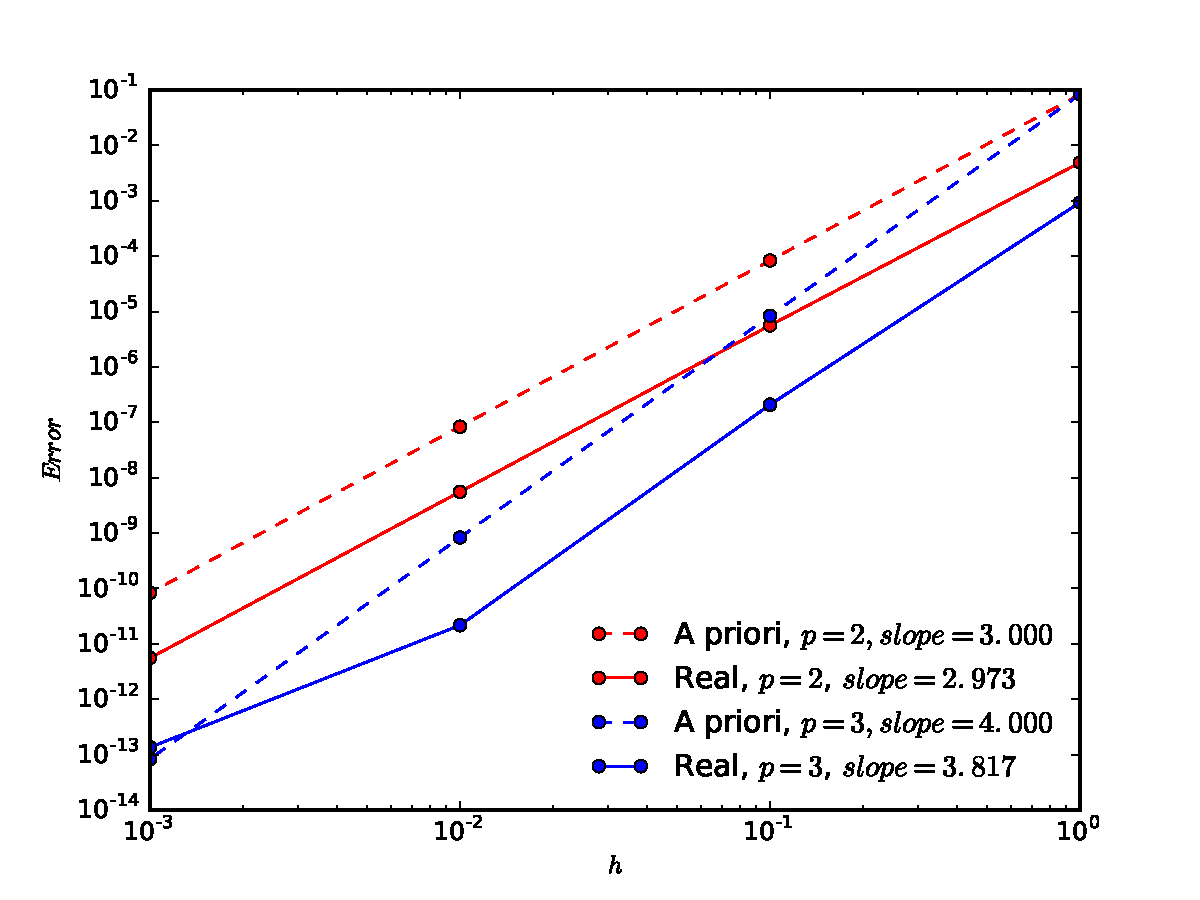
\includegraphics[width=0.75\textwidth]{error_he}
	\caption{Error versus element length}
	\label{fig:11}
\end{figure}

\subsection{}
A plot of the error versus the number of nodes is shown in \cref{fig:12}.
\begin{figure}[ht]
	\centering
	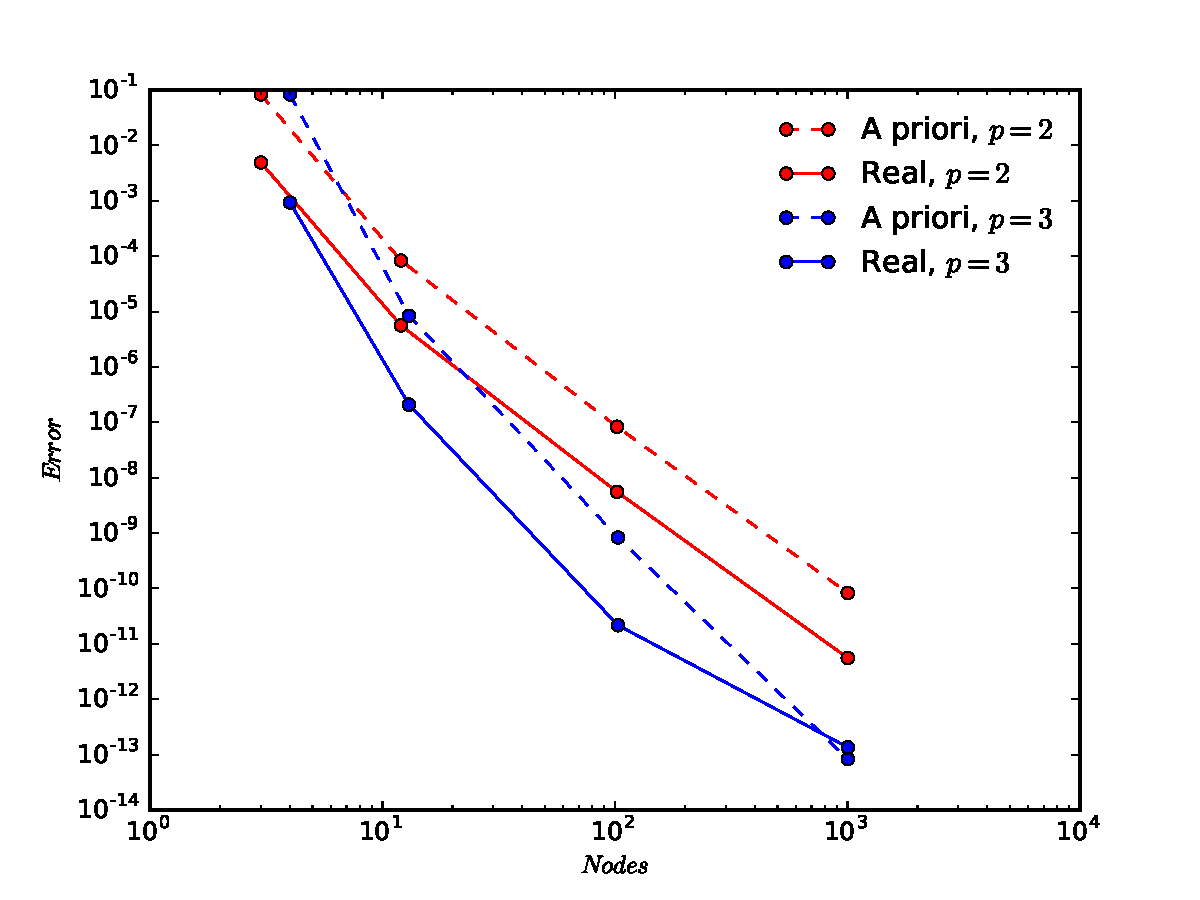
\includegraphics[width=0.75\textwidth]{error_nodes}
	\caption{Error versus the number of nodes}
	\label{fig:12}
\end{figure}

\section{Part 2}

\subsection{}
A plot of deflection versus the number of nodes is provided in \cref{fig:21}. The code is unable to calculate the exact tip deflection using a basis of only order 2 or 3, while the basic beam theory solution is of order 4. By using a higher order basis, such as order 4, the exact deflection could be computed.
\begin{figure}[ht]
	\centering
	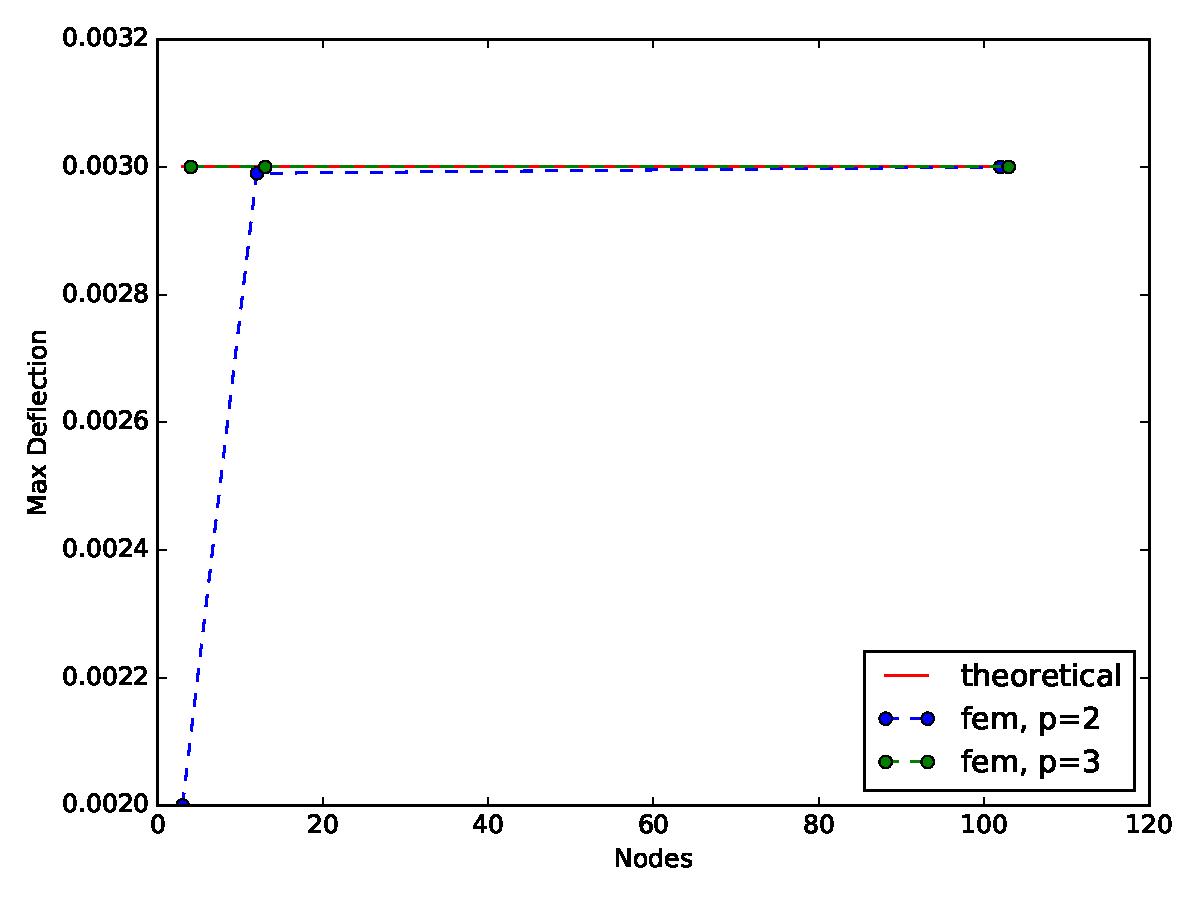
\includegraphics[width=0.75\textwidth]{max_deflection_vs_n}
	\caption{Max deflection vs. the number of nodes}
	\label{fig:21}
\end{figure}

\subsection{}
A plot of dflection versus the beam slenderness is given in \cref{fig:22}. From this plot we can conclude that our method is insensitive to changes in beam slenderness.
\begin{figure}[ht]
	\centering
	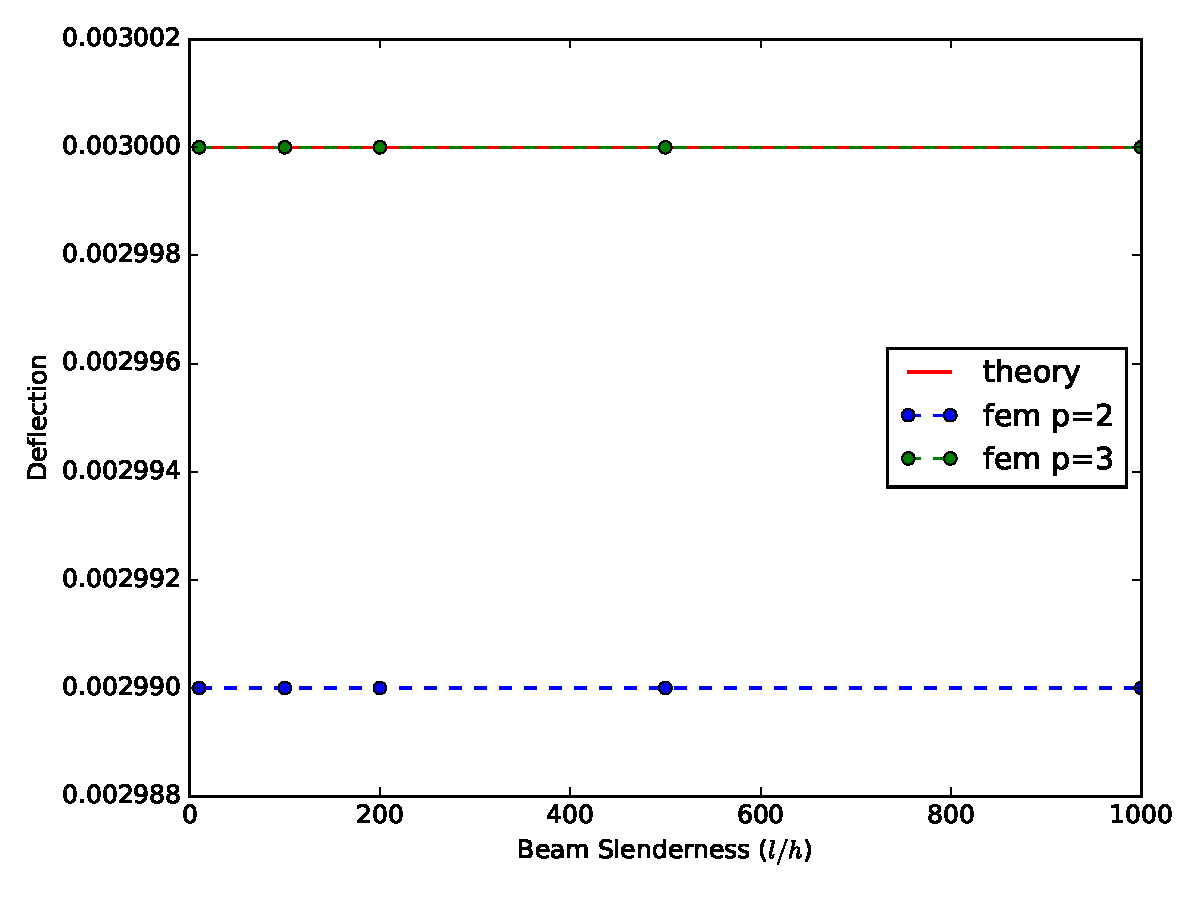
\includegraphics[width=0.75\textwidth, trim={0cm, 0cm, 0cm, 0cm}]{max_deflection_vs_h}
	\caption{Max deflextion vs. the beam slenderness}
	\label{fig:22}
\end{figure}
\end{document}